% Source - https://tex.stackexchange.com/a/728379

\documentclass[tikz,border=5pt]{standalone}
\usetikzlibrary{nfold, decorations.pathreplacing}
% nfold提供了\pgfoffsetpath命令
\makeatletter
\tikzset{offset/.code=\pgfgetpath\tikz@temp\pgfsetpath\pgfutil@empty\pgfoffsetpath\tikz@temp{#1}}
\makeatother
\tikzset{
    make wide and ticks/ticks/.style={
        draw,decorate, decoration={name=ticks, segment length=+5pt, amplitude=2.5pt}
    },
    make wide and ticks/.style={
        offset={#1}, 
        make wide and ticks/ticks
    }
}
\begin{document}
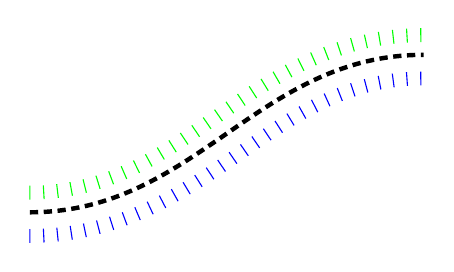
\begin{tikzpicture}
    \draw[ultra thick, densely dashed] (0,0) to[out=0, in=180] (5,2);
    \path[green] (0,0) to[out=0, in=180] (5,2) [make wide and ticks=+ 2.5mm];
    \path[blue] (0,0) to[out=0, in=180] (5,2) [make wide and ticks=+-3mm];
\end{tikzpicture}
\end{document}
